\begin{figure}[htbp]
  \centering
  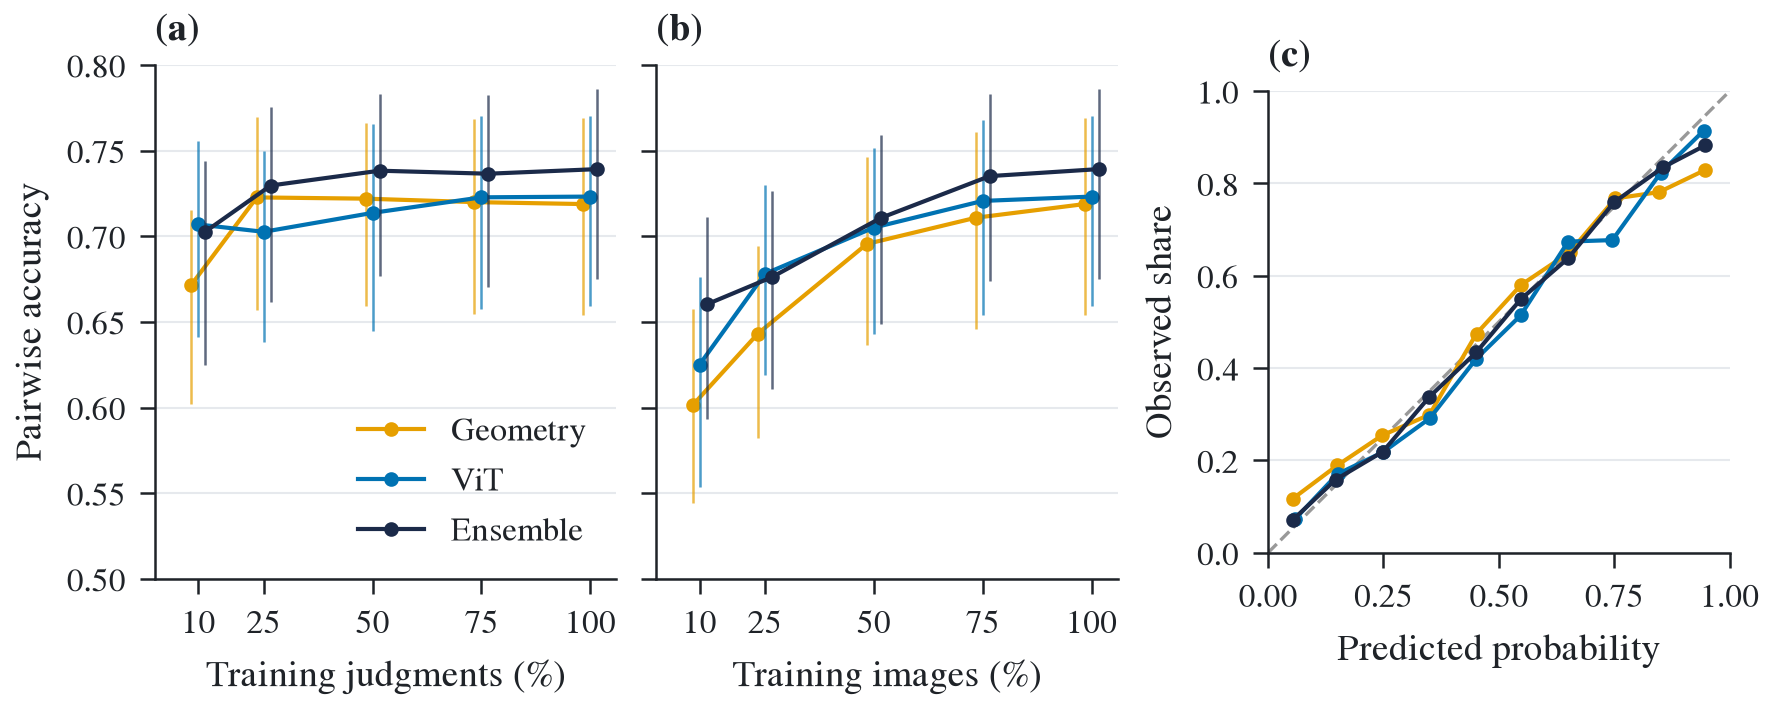
\includegraphics[width=15.00cm]{figures/learning_curves_and_calibration.png}
  \caption{Learning curves and calibration. (a) Accuracy on each fold's test judgments when the methods are trained on a share of the fold's training judgments (all of them, 4,515 on average) between all its training images; (b) on a share of its training images (357 on average), with the judgments between them; the mean over the folds, with 95\% intervals from 1,000 resamples of the manuscripts as bands. (c) Calibration of the predicted win probabilities: per tenth of the predicted probability that the left page is chosen, the share of the test judgments that chose it; the dashed diagonal is perfect calibration. \emph{Geometry}, the pairwise logistic model on the 83 geometric features; \emph{ViT}, the local scoring head on the patch tokens of DINOv2 ViT-S/14 (block 12, 518 pixels on the long edge, the folio crop): an MLP (384--128--1, ReLU, softplus) scoring each patch, the page's score the mean of its patches', trained with RankNet's logistic loss (180 epochs of Adam); \emph{Ensemble}, the mean of the z-scored page scores of \emph{Geometry} and \emph{ViT}. Each method is evaluated by 10-fold cross-validation repeated 10 times, each manuscript's pages in one fold; a fold tests the judgments between two of its pages.}
  \label{fig:learning_curves_and_calibration}
\end{figure}
